\chapter[Números Enteros]{Números Enteros}\label{cap.numeros_enteros}

\begin{section}{Aritmética}\label{seccion-aritmetica}
 Todo lector de este apunte conoce los \textit{enteros}. En una etapa muy temprana de nuestras vidas conocemos los números enteros positivos o ``números naturales'' $$1,2,3,4,5,\ldots$$ Más adelante introducimos el $0$ (cero), y los enteros negativos $$ -1,-2,-3,-4,-5,\ldots $$ 

En este curso no nos preocupamos demasiado por el significado lógico y filosófico de estos objetos, pero necesitamos saber las propiedades que se supone que tienen. Si todos parten de las mismas suposiciones entonces todos llegarán a los mismos resultados. Estos supuestos son los llamados axio\-mas.

El punto de vista adoptado en este apunte es el señalado antes. Aceptamos sin reparo que existe un conjunto de objetos llamados \textit{enteros} conteniendo los enteros positivos y los negativos, y el cero, familiares en nuestra temprana educación y experiencia. El conjunto de enteros se denotará por el símbolo especial ${\mathbb Z}$. Las propiedades de ${\mathbb Z}$ serán dadas por una lista de axiomas, a partir de las cuales seremos capaces de deducir todos los resultados sobre números enteros que necesitaremos en las cuestiones subsiguientes. Empezaremos listando aquellos axiomas que tratan la suma y la multiplicación.

Adoptaremos las notaciones usuales $a+b$ para la suma de dos enteros $a$ y $b$, y $a \cdot b$ (frecuentemente $ab$ o también $a \times b$) para su producto. Pensamos en $+$ y $\cdot$ como \textit{operaciones} que a un par de enteros $a$ y $b$ les hacen corresponder un entero $a+b$ y otro $a\cdot b$. El hecho de que $a \cdot b$ y $a+b$ son enteros, y no algún objeto extra\~no como elefantes, es nuestra primera suposición, el axioma \ref{axioma-i1}.     

En la siguiente lista de axiomas $a$, $b$, $c$ denotan enteros arbitrarios, y $0$ y $1$ denotan enteros especiales que cumplen las propiedades especificadas más abajo.

%\begin{enumerate}[label=\textbf{\arabic*)}, ref=\textbf{\arabic*}]
\begin{enumerate}[label=\textbf{I\arabic*)}, ref=\textbf{I\arabic*}]
\item \label{axioma-i1} $a+b$ y $a\cdot b$ pertenecen a ${\mathbb Z}$.
\item \label{axioma-i2} {\em Conmutatividad.}\, $a+b = b+a$;\qquad $ab=ba$. 
\item \label{axioma-i3} {\em Asociatividad.}\, $(a+b)+c = a+(b+c)$;\qquad $(a\cdot b)\cdot c = a\cdot (b\cdot c)$. 
\item \label{axioma-i4} {\em Existencia de elemento neutro.}\, Existen números $0$, $1 \in \mathbb Z$ con $0\not=1$ tal que $a+0=a$;\qquad $a\cdot 1=a$. 
\item \label{axioma-i5} {\em Distributividad.}\, $a\cdot (b+c)=a\cdot b+a\cdot c$. 
\item \label{axioma-i6} {\em Existencia del inverso aditivo, también llamado opuesto.}\, Por cada $a$ en ${\mathbb Z}$ existe un único entero $-a$ en ${\mathbb Z}$ tal que $a+(-a)=0$. 
\item \label{axioma-i7} {\em Cancelación.}\, Si $a$ es distinto de $0$ y $a\cdot b=a\cdot c$, entonces $b=c$. 
\end{enumerate}


Debido a la ley de asociatividad para la suma, axioma \ref{axioma-i3}, $(a+b)+c$ es igual a $a+(b+c)$ y por lo tanto podemos eliminar los paréntesis sin ambigüedad. Es decir, denotamos
$$
a+b+c := (a+b)+c = a+(b+c).
$$
De forma análoga, usaremos la notación
$$
abc = (ab)c = a(bc).
$$
Debido a la ley de conmutatividad, axioma \ref{axioma-i2}, es claro que  del axioma \ref{axioma-i4} se deduce que  $0+a=a+0=a$ y $1\cdot a = a\cdot 1=a$. Análogamente,  por  \ref{axioma-i2} e  \ref{axioma-i6} obtenemos que  $-a+a =    a+(-a)=0$.

Una propiedad que debemos mencionar es la siguiente: si $a,b, c \in \mathbb Z$  y $a=b$, entonces $a+c = b+c$ y $ac = bc$. Esto se debe a que la suma y el producto son operaciones que, como acabamos de decir, toman un par de enteros y  devuelven otro entero. Si $a=b$, entonces el  par $a,c$ es igual al par $b,c$ y por lo tanto devuelven la misma suma y el mismo producto. Esta propiedad no es un axioma, sino  una mera aplicación de la lógica formal. 
  
Todos los axiomas corresponden a propiedades familiares de los  enteros que aprendemos en distintos niveles de nuestra educación  matemática. De ellas pueden deducirse la mayoría de las reglas  aritméticas comunes de los enteros como en el siguiente ejemplo.

\begin{ejemplo}\label{Ej.opuesto_opuesto} Demostremos que, para todo $n$ entero, el opuesto de $-n$ es $n$, es decir que 
$$-(-n) = n.$$ 
\end{ejemplo}
\begin{proof} El axioma \ref{axioma-i6} nos dice que $-(-n)$ es el único número que sumado a $-n$, da cero.  Por lo tanto, para demostrar que $-(-n) = n$ basta ver que $(-n)+n=0$. Esto se cumple puesto que 
\begin{alignat*}2
(-n)+n&=n+(-n) &\qquad &\text{axioma \ref{axioma-i2}} \\
&=0&\qquad &\text{axioma \ref{axioma-i6}}
\end{alignat*}
Por lo tanto  $(-n)+n=0$.
\end{proof}

Como ya dijimos, los números enteros vienen provistos con dos operaciones fundamentales, la suma y la multiplicación.
A continuación definimos la resta o sustracción. 

\begin{definicion} Si $a,b\in\mathbb{Z}$ definimos $a-b$ como la suma de $a$ más el opuesto de $b$, es decir que  $a-b=a+(-b)$ por definición.  
\end{definicion}

Ahora demostremos una propiedad básica de la resta.

\begin{ejemplo*} Demostremos que para dos enteros $m$ y $n$ cualesquiera
$$m-(-n) = m+n.$$ 
\end{ejemplo*}
\begin{proof} Por la definición de sustracción, $m-(-n)$ es la suma $m+(-(-n))$, es decir 
$$m-(-n)=m+(-(-n)).$$ 
Por el ejemplo \ref{Ej.opuesto_opuesto} sabemos que $-(-n)=n$ y por lo tanto $m-(-n)=m+(-(-n))=m+n$.
\end{proof}

Tanto formalismo, como el usado en las  demostraciones realizadas en el ejemplo anterior, puede ser tedioso, pero nos permiten comenzar a comprender la estructura de una demostración formal. 



\begin{ejemplo*} Supongamos que existen dos enteros $0$ y $0'$ ambos cumpliendo el  axioma \ref{axioma-i4}, esto es
$$
a+0= a, \qquad a+0'=a
$$
para todo $a$ de $\mathbb Z$.  Entonces $0= 0'$. 
\end{ejemplo*}
\begin{proof}
\begin{alignat*}2
0 &= 0 + 0'&\qquad &\text{axioma \ref{axioma-i4} aplicado a $0$ y con $0'$ como neutro} \\
&=0'+0&\qquad &\text{axioma \ref{axioma-i2}}\\
&= 0' &\qquad &\text{axioma \ref{axioma-i4} aplicado a $0'$ y con $0$ como neutro}.
\end{alignat*}
\end{proof}


El ejemplo anterior nos demuestra que hay un único elemento elemento que cumple el axioma \ref{axioma-i4} en lo que respecta a la suma. A este elemento lo denotamos $0$ y lo denominamos el {\em elemento neutro de la suma}. Lo mismo podemos probar con el elemento neutro respecto al producto (ver ejercicio \ref{ej-elem-neutro-prod}),  es decir hay un único elemento,  denotado 1, que satisface el axioma \ref{axioma-i4} en lo que se refiere al producto. A  este elemento lo llamamos el {\em elemento neutro del producto}.  

\begin{ejemplo*} (Regla de los signos) Veamos que  si $a,b \in \mathbb Z$ entonces
$$
(-a)(-b) = ab ,\qquad a(-b) = (-a)b = -(ab).
$$
\end{ejemplo*}
\begin{proof}
Veremos que  $a(-b) = -(ab)$. Los otros casos se dejan como ejercicio para el lector.

Una forma de demostrar este caso es  observando que $-(ab)$ es el inverso aditivo de $ab$ y comprobando que $a(-b)$ es también inverso aditivo de $ab$. Luego, por unicidad del inverso aditivo, de deduce que $a(-b) = -(ab)$. 
\begin{alignat*}2
ab + a(-b) &=a(b-b) &\qquad &\text{axioma \ref{axioma-i5}} \\
&=a0 &\qquad &\text{axioma \ref{axioma-i4}}\\
&= 0 &\qquad &\text{ejercicio \ref{ej0a}}.
\end{alignat*}
Es decir $a(-b)$ es el inverso aditivo de $ab$, luego por la unicidad del inverso aditivo axioma \ref{axioma-i6}, $a(-b)=-(ab)$.
\end{proof}


Algunos resultados similares pueden encontrarse en los siguientes ejercicios. Como aún no tenemos todos los axiomas correspondientes a los enteros, los resultados no son particularmente interesantes, pero lo que importa es recordar que pueden ser probados sobre la base única de los axiomas.


\subsection*{$\S$ Ejercicios}

\begin{enumex}
\item Demostrar la regla $(a+b)c=ac+bc$, explicando cada paso.

\item Como siempre $x^2$ denota $x\cdot x$. Demostrar que dados dos enteros $a$ y $b$ tal que $a+b \not=0$, entonces existe un único $c$ tal que $(a+b)c=
a^2 - b^2$.

\item \label{ej-elem-neutro-prod} Probar que hay un único elemento neutro del producto.

\item \label{ej0a}
La siguiente es una demostración de la fórmula $0x=0$ usando solo los axiomas planteados antes. Escribir la demostración completa, explicando que axioma es usado en cada paso.
$$\begin{aligned}
0x &= (0+0)x &\qquad &\mbox{axioma (.....)}\\  
&=0x+0x. &\qquad &\mbox{axioma (.....)}
\end{aligned}$$
Luego $0x =0x+0x$. Sumando $-0x$ a ambos miembros de la igualdad, obtenemos 
$$\begin{aligned}
0x +(-0x) &= 0x+0x+(-0x) &\qquad &\mbox{(usando lógica formal)}\\  
0 &= 0x+0 &\qquad &\mbox{axioma (.....), 2 veces}\\  
0 &=0x. &\qquad &\mbox{axioma (.....)}
\end{aligned}$$
\end{enumex}

\end{section}



\begin{section}{Ordenando los enteros}\label{seccion-ordenando-los-enteros}

El orden natural de los enteros es tan importante como sus propiedades aritméticas. Desde el comienzo aprendemos los números en el orden $1, 2, 3, 4, 5,$ y el hecho de que $4$ es ``mayor'' que $3$ se convierte en algo de importancia práctica para nosotros. Expresamos esta idea formalmente diciendo que existe una relación que indicamos ``$<$'' ($a < b$ se lee: $a$ es menor que $b$ o también $b$ es mayor que $a$). 

Solo cuatro axiomas se necesitan para especificar las propiedades básicas del símbolo $<$ , y ellos son listados en lo que sigue. La numeración de los axiomas se continúa de la sección \ref{seccion-aritmetica}. Como antes, $a$, $b$ y $c$ denotan enteros arbitrarios.

\begin{enumerate}[label=\textbf{I\arabic*)}, ref=\textbf{I\arabic*}]
    \setcounter{enumi}{7}
    \item \label{axioma-i8} {\em Ley de tricotomía.}\, Vale una y sólo una de las relaciones
siguientes:
$$
a<b, \qquad a = b, \qquad b < a.
$$
\item \label{axioma-i9} {\em Ley transitiva.}\, Si $a< b$ y $b < c$, entonces $a<c$.
\item \label{axioma-i10} {\em Compatibilidad de la suma con el orden.}\, Si $a < b$, entonces $a+c < b+c$. 
\item \label{axioma-i11} {\em Compatibilidad del producto con el orden.}\, Si $a< b$ y $0< c$, entonces $ac < bc$. 
\end{enumerate}


Esta claro que podemos definir los otros símbolos de orden $>$, $\le$ y $\ge$, en términos de los símbolos $<$ e $=$. Diremos que $m>n$ si  $n<m$, diremos que $m \le n$ si $m<n$ o $m=n$. Finalmente, diremos que $m \ge n$ si $m > n$ o $m=n$.  Es importante notar que el  axioma \ref{axioma-i11} tiene una versión valedera para estos nuevos símbolos.
\begin{enumerate}[label=\textit{\alph*)}]
\item \textbf{($>$)} Si $a > b$ y $c>0$, entonces $ac > bc$.
\item \textbf{($\le$)} Si $a \le b$ y $0 \le c$, entonces $ac \le bc$.
\item \textbf{($\ge$)} Si $a\ge b$ y $c\ge 0$, entonces $ac \ge bc$.
\end{enumerate}
Usando las definiciones de $\ge$, $<$, $>$ y el axioma \ref{axioma-i11} original es muy sencillo demostrar estas variantes. Por otro lado,

\begin{proposicion}\label{prop-compatibilidad-negativa}
    Sean $a, b, c \in \Z$.  
    \begin{enumerate}[label=\textit{\alph*)}]
        \item\label{it.cmenor0} Si $c < 0$, entonces $0 < -c$.
        \item\label{it.amenorb} Si $a< b$ y $c< 0$, entonces $ac > bc$. 
    \end{enumerate}
\end{proposicion}
\begin{proof}[Demostración (*)] {${}^{}$}
    
    \ref{it.cmenor0} Sumando $-c$ a ambos miembros de la desigualdad $c < 0$, obtenemos $c + (-c) < 0 + (-c)$ (compatibilidad de la suma con la relación de orden). Por los axiomas de inverso aditivo y elemento neutro, la expresión se reduce a $0 < -c$.
    
    \ref{it.amenorb} Como $a < b$, si sumamos a ambos miembros de la desigualdad $-a -b$, por la compatibilidad  de la suma con $<$, obtenemos $a -a -b < b -a -b$ y por la aplicación reiterada de los axiomas de inverso aditivo y elemento neutro  obtenemos $-b < -a$. Por a) sabemos que $0< -c$, por lo tanto, por \ref{axioma-i11}, $(-b)(-c) < (-a)(-c)$. Aplicando la regla de los signos obtenemos $bc < ac$ y por lo tanto $ac > bc$.

\end{proof}

Ya hemos usado (en axioma \ref{axioma-i4}) el símbolo $\not=$ que denota  ``{\em no} es igual a '' o bien ``es distinto a''.   En  general, cuando tachemos un símbolo, estamos indicando la negación de la relación que define. Por ejemplo, $a\not< b$ denota ``$a$ {\em no} es menor que $b$''. 

\begin{observacion*} Demostremos que  $a\not< b$ es equivalente a $a\ge b$: por la ley de tricotomía axioma \ref{axioma-i8} tenemos que solo vale una y solo una de las siguientes afirmaciones
$$
a<b, \qquad a = b, \qquad b < a.
$$
Como  $a\not< b$, entonces vale una de las dos afirmaciones siguientes, $a=b$ o $b<a$, es decir  vale que $a \ge b$. De forma análoga se prueba que $a\not\le b$ si  y sólo si $a>b$, $a\not> b$ si  y sólo si $a \le b$ y $a\not\ge b$ si  y sólo si $a<b$.

\end{observacion*}


\begin{ejemplo}\label{relaciondeorden}
Demostremos las siguiente propiedades de $\le$. Sean  $a$, $b$ y $c$  enteros arbitrarios,  entonces
\begin{enumerate}
\item[\textbf{O1)}] {\em Reflexividad.}\, $a \le a$.
\item[\textbf{O2)}] {\em Antisimetría.}\, Si $a \le b$ y $b \le a$, entonces $a=b$.
\item[\textbf{O3)}] {\em Transitividad.}\, Si $a\le b$ y $b\le c$, entonces $a \le c$.
\end{enumerate}
\begin{proof}
\
    
(\textbf{O1}) Como $a=a$, tenemos entonces que $a \le a$ (por definición de $\le$).


(\textbf{O2}) Como $a \le b$, tenemos que $a<b$ o bien $a=b$ (por tricotomía no pueden valer ambas). Si ocurriera que $a<b$, por la observación anterior, tendríamos que $a\not\ge b$, es decir $b\not\le a$, lo cual es absurdo pues una de nuestras hipótesis es,  justamente, lo contrario:  $b \le a$.  Es decir, la única posibilidad que queda es que $a=b$.     

%\vskip .2cm
(\textbf{O3}) Como $a\le b$, entonces $a <b$ o bien $a=b$. Como $b\le c$, entonces $b<c$ o bien $b=c$. Para hacer la demostración, debemos pensar en todas las posibles combinaciones de estas afirmaciones:
\begin{itemize}
    \item $a<b$ y $b<c$. Es este caso, por  \ref{axioma-i9}, $a<c$. Luego $a\le c$.
    
    \item $a<b$ y $b=c$. Luego $a<c$ y eso implica que $a\le c$.
    
    \item $a=b$ y $b<c$. Luego $a<c$ y eso implica que $a\le c$.
    
    \item $a=b$ y $b=c$. Es claro entonces que $a=c$, lo cual implica que $a\le c$.
\end{itemize}    
\end{proof}
\end{ejemplo}

Una relación que satisfaga las tres propiedades anteriores (reflexividad, antisimetría y transitividad) es llamada {\em una relación de orden}. Observar que $<$ {\em no} es una relación de orden, en el sentido de la definición anterior. 

A primera vista podría parecer que ya tenemos todas las propiedades que necesitamos de $\mathbb Z$, pero, sorprendentemente, aún falta un axioma de vital importancia. Supongamos que $X$ es un subconjunto de $\mathbb Z$; entonces diremos que el entero $b$ es una {\em cota inferior}\index{cota inferior} de $X$ si
$$
b\le x \qquad \text{ para todo } \ x \in X.
$$
Algunos subconjuntos no tienen cotas inferiores: por ejemplo, el conjunto de los enteros negativos $-1, -2, -3, \ldots$, claramente no tiene cota inferior. Por otro lado, el conjunto $S$ denotado por los números resaltados en la Fig. \ref{f1.1} tiene muchas cotas inferiores. Una mirada rápida nos dice que $-9$ por ejemplo es una cota inferior, mientras que una inspección más minuciosa revela que $-7$ es la ``mejor'' cota inferior, pues en realidad pertenece a $S$. En general, una cota inferior de un conjunto $X$ que es a su vez es un elemento de $X$, es conocido como el {\em mínimo}\index{mínimo} de X.

%\vskip .3cm


\begin{figure}[ht]
$$
-10, -9, -8, \mathbf{-7}, \mathbf{-6}, -5, -4, \mathbf{-3}, -2, -1, 0, \mathbf{1}, \mathbf{2}, \mathbf{3}, 
4, 5, 6, 7, 8, 9, 10
$$
\caption{El mínimo de $S$ es $-7$.}\label{f1.1}
\end{figure}
%\vskip .3cm


Nuestro último axioma para $\mathbb Z$ afirma algo que es (aparentemente) una propiedad obvia.
\begin{enumerate}[label=\textbf{I\arabic*)}, ref=\textbf{I\arabic*}]
    \setcounter{enumi}{11}
    \item \label{axioma-i12} Si $X$ es un subconjunto de $\mathbb Z$ que no es vacío y tiene una cota inferior, entonces $X$ tiene un mínimo.
\end{enumerate}

El axioma \ref{axioma-i12} es conocido como el  \textit{axioma de buena ordenación}  o  \textit{axioma del buen orden}\index{axioma del buen orden} o \textit{principio de buena ordenación}\index{principio de buena ordenación}.  Una buena forma de entender su significado es considerar $X$ un conjunto de enteros acotado inferiormente  y un juego en el cual dos personas eligen alternativamente un elemento de $X$, sujetos a la regla de que cada número debe ser estrictamente menor que el anterior. El axioma nos dice que cuando los números son enteros, el juego terminará; además el final se producirá cuando uno de los jugadores tenga el buen sentido de elegir el mínimo. Esta propiedad aparentemente obvia \textit{no} se mantiene necesariamente cuando tratamos con números que no son enteros, pues $X$ puede no tener un mínimo aunque tenga una cota inferior. Por ejemplo supongamos que $X$ es el conjunto de fracciones $3/2, 4/3, 5/4, \ldots$ teniendo por forma general $(n+1)/n$, $n\ge 2$. Este conjunto tiene una cota inferior ($1$, por ejemplo) pero no tiene mínimo y por lo tanto los jugadores podrían seguir jugando para siempre, eligiendo fracciones más y más cercanas a $1$.

El axioma del buen orden nos da una justificación firme para nuestro intuitivo dibujo de los enteros: un conjunto de puntos regularmente espaciados sobre una linea recta, que se extiende indefinidamente en ambas direcciones como en la Fig. \ref{f1.2}. En particular dice que no podemos acercarnos más y más a un entero sin alcanzarlo, de forma que el dibujo de la Fig. \ref{f1.3} no es correcto.

\begin{figure}[ht]
    \begin{center}
    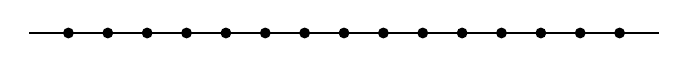
\begin{tikzpicture}[line width=1pt]    
    \draw (-4.0,0) -- (4.0,0); 
    \foreach \x in {-7,...,7}
    \draw [fill] (\x/2,0) circle [radius=0.05];
    \end{tikzpicture}
    \end{center}
    \caption{El dibujo correcto de $\mathbb Z$.}\label{f1.2}
\end{figure}

\begin{figure}[ht]    
    \begin{center}
    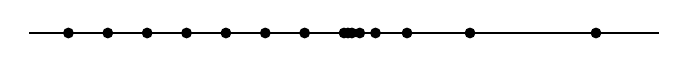
\begin{tikzpicture}[line width=1pt]    
    \draw (-4.0,0) -- (4.0,0); 
    \foreach \x in {-7,...,0}
    \draw [fill] (\x/2,0) circle [radius=0.05];
    \foreach \x in {0.05,0.1,0.2,0.4,0.8,1.6,3.2}
    \draw [fill] (\x,0) circle [radius=0.05];
    \end{tikzpicture}
    \end{center}
    \caption{El dibujo incorrecto de $\mathbb Z$.}\label{f1.3}
\end{figure}

El hecho de que haya espacios vacíos entre los enteros nos lleva a decir que el conjunto $\mathbb Z$ es \textit{discreto} y es esta propiedad la que da origen al nombre ``matemática discreta''. En cálculo y análisis, los procesos de límite son de fundamental importancia, y es preciso usar aquellos sistemas numéricos que son \textit{continuos}, en vez de los discretos.

El siguiente resultado es obvio, pero  debe ser demostrado. Sin embargo,  la demostración es bastante compleja y sólo se da por completitud. 
\begin{proposicion}\label{prop-0-menor-que-1}
$1$ es el menor entero mayor que $0$.
\end{proposicion}
\begin{proof}[Demostración (*)] Primero debemos probar que $0 < 1$. Ahora bien, como $0 \not= 1$ (por axioma \ref{axioma-i4}), por la ley de tricotomía (axioma \ref{axioma-i8}), debe ocurrir que $0 < 1$ o $ 1 < 0$. Supongamos que $1 < 0$, luego por proposición \ref{prop-compatibilidad-negativa}, $1 \cdot 1 > 1 \cdot 0$. Como $1$  es elemento neutro de la multiplicación, obtenemos $1 > 0$, que contradice nuestra suposición. Esta contradicción vino de suponer que $1 < 0$. Por lo tanto, $0 < 1$.

Probaremos ahora que no existe $a$ entero tal que $ 0<a<1$ y lo haremos por el absurdo: supongamos que existe $a \in \mathbb Z$ tal que $0<a<1$ y sea 
$$
X=\{a\in\mathbb Z: 0<a<1\}.
$$
La  suposición que hicimos implica que $X$ es no vacío.  Dado que todos los elementos de $X$ son positivos, $X$ es un subconjunto de $\mathbb Z$ acotado inferiormente ($0$ es cota inferior). Por el axioma del buen orden\ref{axioma-i12} resulta que $X$ tiene un elemento mínimo, que llamaremos $a_0$, y cumple
$$
0<a_0<1. 
$$
Usamos ahora la compatibilidad del  producto con  la relación de orden \ref{axioma-i11}:  por un lado multiplicamos por $a_0$ la desigualdad $0<a_0$ y obtenemos $0<a_0^2$,  y por otro lado multiplicamos por $a_0$ la desigualdad $a_0<1$ y obtenemos $a_0^2<a_0$. Es decir
$$
 0<a_0^2<a_0<1.
$$
La desigualdad $0<a_0^2<1$ dice que $a_0^2\in X$ pero la desigualdad $a_0^2<a_0$ dice que  $a_0$ no es el mínimo elemento de $X$, lo cual es una contradicción pues dijimos que $a_0$ es el mínimo elemento de $X$.  El  absurdo  vino de suponer que existe $a \in \mathbb Z$ tal que   $0<a<1$.
\end{proof}


\subsection*{$\S$ Ejercicios}
\begin{enumex}
    \item Demostrar que $\ge$ es una relación de orden.
        
    \item Demostrar que dados cualesquiera $a,b,c \in \mathbb Z$ vale que si $a< b$ y $0\le c$, entonces $ac \le bc$. 
        
    \item Demostrar que si $a\le b$ y $c\le 0$, entonces $bc \le ac$.
        
    \item Demostrar que $0\le x^2$ para todo $x$ en $\mathbb Z$.
        
    \item Deducir de la proposición \ref{prop-0-menor-que-1} que $n+1$ es el menor entero mayor que $n$ para todo $n$ en $\mathbb Z$.

    \item Demostrar que si un conjunto $X$ tiene mínimo, este es único. Dicho más formalmente: demostrar que si existen $c,c' \in X$ tal que  $c\le x$ y $c'\le x$ para todo $x \in X$, entonces $c=c'$. 

    \item En cada uno de los siguientes casos decir si el conjunto $X$ tiene o no una cota inferior, y si la tiene, encontrar el mínimo.
    \begin{enumerate}
        \item $X = \{x \in \mathbb Z | x^2\le 16\}.$
        \item $X =\{x \in \mathbb Z | x=2y \text{\ para algún } y \in \mathbb Z\}.$
        \item $X =\{x \in \mathbb Z | x\le 100\,x\} .$
    \end{enumerate}
    \item Un subconjunto $Y$ de $Z$ se dice que tiene una {\em cota superior}\index{cota superior} $c$ si $c\ge y$ para todo $y \in Y$.  Una cota superior que además es un elemento de $Y$ es llamada el {\em máximo} de $Y$. Usar el axioma \ref{axioma-i12} para demostrar que si $Y$ es no vacío y tiene una cota superior, entonces tiene máximo. [Ayuda: aplicar el axioma al conjunto cuyos elementos son $-y$ ($y \in Y$).]

    \item Los enteros $n$ que satisfacen $1 \le n \le 25$ están acomodados en forma arbitraria en un arreglo cuadrado de cinco filas y cinco columnas. Se selecciona el máximo  de cada fila, y se denota $s$ al mínimo entre ellos. De manera similar, el mínimo de cada columna es seleccionado y $t$ denota al máximo entre ellos. Demostrar que $s\ge t$ y de un ejemplo en el cual $s\not=t$.
\end{enumex}

\end{section}

\begin{section}{Definiciones recursivas}\label{seccion-definiciones-recursivas}

Sea $\mathbb N$ el conjuntos de enteros positivos, esto es
$$
\mathbb N = \{ n \in \mathbb Z | n\ge 1\},
$$
y denotemos $\mathbb N_0$ el conjunto $\mathbb N \cup \{0\}$, esto
es
$$
\mathbb N_0 = \{ n \in \mathbb Z | n\ge 0\}.
$$
$\mathbb{N}$  es llamado el conjunto de  \textit{números naturales}. Si $X$ es un subconjunto de $\mathbb N$ (o de $\mathbb N_0$)  entonces automáticamente tiene una cota inferior, pues cada elemento $x$ de $X$ satisface $x\ge 1$ (o $x\ge 0$). As{í}, en este caso el axioma del buen orden toma la forma
$$
\begin{aligned}
&\textit{si $X$ es un subconjunto no vacío de $\mathbb N$ o $\mathbb N_0$ entonces $X$
 tiene un mínimo.}
\end{aligned}
$$
Esta la forma más usada en la práctica.

Nuestro primer uso del axioma del buen orden será para justificar un procedimiento muy usual. Frecuentemente encontramos una expresión de la forma $u_n$, donde $n$ indica cualquier entero positivo: por ejemplo, podríamos tener $u_n=3n+2$, o $u_n = (n+1)(n+2)(n+3)$. En estos ejemplos $u_n$ es dado por una fórmula explícita y no existe dificultad en calcular $u_n$ cuando se nos da un valor específico para $n$. Sin embargo en muchos casos no conocemos una fórmula para $u_n$; es más, nuestro problema puede ser encontrarla. En estos casos pueden darnos ciertos valores de $u_n$ para enteros positivos $n$ peque\~nos, y una relación entre el $u_n$ general y algunos de los $u_r$ con $r<n$. Por ejemplo, supongamos nos es dado 
$$ 
u_1=1, \qquad u_2=2, \qquad u_n =u_{n-1} +u_{n-2}, \qquad n\ge 3.
$$
Para calcular los valores de $u_n$ para todo $n$ de $\mathbb N$ podemos proceder como sigue:
$$
\begin{matrix}
u_3 & = & u_2 + u_1 & = & 2+1 &=& 3, \\
u_4 & = & u_3 + u_2 & = & 3+2 &=& 5, \\
u_5 & = & u_4 + u_3 & = & 5+3 &=& 8,
\end{matrix}
$$
y así siguiendo.  Éste es un ejemplo de una \textit{definición recursiva}. Es ``obvio'' que el método dará un valor único de $u_n$ para todo entero positivo $n$. Pero hablando estrictamente necesitamos el axioma del buen orden para justificar la conclusión a través de las siguientes líneas.

Supongamos que existe un entero positivo $n$ para el cual $u_n$ no está definido de manera única. Entonces por el axioma del buen orden existe un entero positivo mínimo $m$ con esta propiedad. Como $u_1$ y $u_2$ están explícitamente definidos, $m$ no es $1$ o $2$ y la ecuación $u_m =u_{m-1} +u_{m-2}$ es aplicable. Por la definición de $m$, $u_{m-1}$ y $u_{m-2}$ están definidos de manera única, y la ecuación nos da un valor único para $u_m$ , contrariamente a la hipótesis. La contradicción surge de suponer que no está bien definido para algún $n$, y por lo tanto esta suposición debe ser falsa.

El lector no debe desanimarse por el uso de argumentos tan retorcidos para establecer algo que es ``obviamente'' verdadero. En primer lugar, no debemos usar resultados ilegítimamente (sin demostrarlos), y en segundo lugar, el hecho de que el resultado sea ``obvio'' simplemente indica que estamos trabajando con la correcta representación mental de $\mathbb N$ y $\mathbb Z$. Una vez que hemos establecido esa representación sobre bases firmes podemos empezar a extendernos y obtener resultados que no sean tan ``obvios''.

El método de definición recursiva aparecerá bastante seguido en el resto del apunte. Existen otras formas de este procedimiento que se ``esconden'' por su notación. ¿Qué significan las siguientes expresiones?
$$
\sum_{r=1}^{n} 2r-1,\qquad 1+3+5+\cdots +(2n-1).
$$
Claramente no basta decir que uno significa lo mismo que el otro, porque cada uno contiene un misterioso símbolo, $\sum$ y $\cdots$, respectivamente. Lo que deberíamos decir es que cada uno de ellos es equivalente a la expresión $s_n$, dada por la siguiente definición recursiva:
$$
s_1= 1, \qquad s_n = s_{n-1} +(2n-1), \qquad n\ge 2.
$$

Esto hace ver claro que ambos símbolos misteriosos son, en realidad, una forma de acortar una definición recursiva, y que por lo tanto son expresiones definidas para todo $n$ en $\mathbb N$.

Ideas similares pueden aplicarse a la definición de productos tal como $n!$ (que se lee $n$ \textit{factorial}). Si decimos que
$$
n!=1 \cdot 2 \cdot 3 \cdots n,
$$
el significado es bastante claro para cualquiera. Pero para precisar (y hacerlo claro para una computadora) debemos usar las definiciones recursivas.

\begin{definicion} Sea $n \in \N$ sean $a_i$  para $1 \le i \le n$, una secuencia de números (enteros, reales, etc.). Entonces $\sum_{i=1}^{n} a_i$  denota la función recursiva definida  
    $$
    \sum_{i=1}^{1} a_i= a_1, \qquad \sum_{i=1}^{n} a_i = \sum_{i=1}^{n-1} a_i+ a_{n} \quad (n\ge 2).
    $$
    En  este caso  decimos que  $\sum_{i=1}^{n} a_i$ es la \textit{sumatoria} de los $a_i$ de $i=1$  a $n$. El símbolo $\prod_{i=1}^{n} a_i$ denota la función recursiva definida  
    $$
    \prod_{i=1}^{1} a_i= a_1, \qquad \prod_{i=1}^{n} a_i = \prod_{i=1}^{n-1} a_i \cdot  a_{n} \quad (n\ge 2).
    $$
    En  este caso  decimos que  $\prod_{i=1}^{n} a_i$ es la \textit{productoria} de los $a_i$ de $i=1$  a $n$. 
\end{definicion}



En  el caso de $n!$ se puede  o bien definir como $\prod_{i=1}^{n} i$, o bien como
$$
1!=1,\qquad n!=n \cdot (n-1)! \quad (n\ge 2).
$$

Otro caso que debemos mencionar es  el de la definición de ``$n$-ésima potencia'': sea $x$ un  número, si $n \in \N$ definimos
$$
x^1=x,\qquad x^n= x \cdot x^{n-1} \quad (n\ge 2).
$$
Por completitud,  definimos $x^0=1$. 

\subsection*{$\S$ Ejercicios}
\begin{enumex}
    \item En el caso siguiente calcule (donde sea posible) los valores de $u_1$, $u_2$, $u_3$ y $u_4$ dados por las ecuaciones. Si no puede calcular los valores explicar porque la definición no esta bien.
    \begin{enumex}
        \item $u_1 = 1$,\qquad $u_2=1$,\qquad $u_n = u_{n-1} +2 u_{n-2}$,\qquad $n \ge 3$. 
        \item $u_1 = 1$,\qquad $u_n = u_{n-1} +2u_{n-2}$,\qquad $n \ge 2$. 
        \item $u_1 = 0$,\qquad $u_n = nu_{n-1}$,\qquad $n \ge 2$.
    \end{enumex}

    \item Sea $u_n$ definido por las ecuaciones
    $$
    u_1=2,\qquad u_n= 2^{u_{n-1}}, \qquad n\ge 2.
    $$
    ¿Cuál es el primer valor de $n$ para el cual no se puede calcular $u_n$ usando una calculadora de bolsillo o de su celular?

    \item Escribir fórmulas explícitas para las expresiones $u_n$ definidas por las siguientes ecuaciones.
    \begin{enumex}
        \item $u_1 = 1$,\qquad $u_n = u_{n-1} +3$,\qquad $n \ge 2$. 
        \item $u_1 = 1$,\qquad $u_n = n^2u_{n-1}$,\qquad $n \ge 2$.
    \end{enumex}
\end{enumex}
\end{section}


\begin{section}{El principio de inducción}\label{seccion-principio-de-induccion}

Supongamos que nos piden que demostremos el resultado
$$
1+3+5+\cdots+(2n-1) = n^2.
$$
En otras palabras, debemos demostrar que la expresión de la izquierda definida recursivamente es igual a la expresión definida explícitamente por la fórmula de la derecha, para todos los enteros positivos $n$. Podemos proceder como sigue.

La fórmula es ciertamente correcta cuando $n=1$ puesto que $1=1^2$.  Supongamos que es correcta para un valor específico de $n$, digamos para $n=k$, de modo que
$$
1+3+5+\cdots+(2k-1) = k^2.
$$
Podemos usar esto para simplificar la expresión definida recursivamente a la izquierda cuando $n$ es igual a $k+1$,
$$
\begin{aligned}
1+3+5+\cdots+(2k+1) &= 1+3+5+\cdots+(2k-1) +(2k+1) \\
&=k^2 +(2k+1) \\
&=(k+1)^2.
\end{aligned}
$$
Por lo tanto si el resultado es correcto cuando $n=k$, entonces lo es cuando $n=k+1$. Se comienza observando que si es correcto cuando $n=1$, debe ser por lo tanto correcto cuando $n=2$. Con el mismo argumento como es correcto cuando $n=2$ debe serlo cuando $n=3$. Continuando de esta forma veremos que es correcto para todos los enteros positivos $n$.

La esencia de este argumento es comúnmente llamada \textit{principio de inducción}. Es una técnica poderosa, fácil de aplicar y la aplicaremos frecuentemente. Pero primero debemos examinar sus bases lógicas y para hacerlo necesitamos una formulación más general. 

Supongamos que queremos demostrar que un resultado es verdadero para todo $n \in \mathbb N$. Con $S$ denotemos al subconjunto de $\mathbb N$ para el cual el resultado es correcto: por supuesto, nuestra intención es probar que $S$ es todo $\mathbb N$. El primer paso es probar que $1$ pertenece a $S$, y luego demostraremos que si $k$ pertenece a $S$, también $k+1$. Entonces lo pensamos paso a paso, un procedimiento infinito, y concluimos que $S=\mathbb N$. Afortunadamente el pensarlo paso a paso no es esencial debido a que el principio de inducción es consecuencia de los axiomas que elegimos tan cuidadosamente para $\mathbb Z$ y $\mathbb N$. Más específicamente es consecuencia del axioma del buen orden.

\begin{teorema}[Principio de inducción]\label{teorema-principio-de-induccion} Supongamos que $S$ es un subconjunto de $\mathbb N$ que satisface las condiciones \index{principio de inducción}
\begin{enumerate}[label=\textit{\alph*)}]
\item\label{caso-base} $1 \in S$,
\item\label{paso-inductivo} para cada $k \in \mathbb N$, si $ k \in S$ entonces $k+1\in S$.
\end{enumerate}
Entonces se sigue que $S=\mathbb N$.
\end{teorema}
\begin{proof}Si la conclusión es falsa, $S \not= \mathbb N$ y
el conjunto complementario $S^{\text{c}}$ definido por
$$
S^{\text{c}}= \{ r \in \mathbb N | r\not\in S\}
$$
 es no vacío. Por el axioma del buen orden, $S^{\text{c}}$ tiene un menor elemento $m$. Como por \ref{caso-base} el $1$ pertenece a $S$, $m\not=1$. Se sigue que $m-1$ pertenece a $\mathbb N$ y como $m$ es el mínimo de $S^{\text{c}}$, $m-1$ debe pertenecer a $S$. Poniendo $k=m-1$ en la condición \ref{paso-inductivo}, concluimos que $m$ esta en $S$, lo cual contradice el hecho de que $m$ pertenece a $S^{\text{c}}$. De este modo, la suposición $S \not= \mathbb N$ nos lleva a un absurdo, y por lo tanto tenemos $S= \mathbb N$. 
 \end{proof}

En la práctica, generalmente presentamos una ``demostración por inducción'' en términos más descriptivos. El hecho de que el resultado es verdadero cuando $n=1$ se llama \textit{base de la inducción} o \textit{caso base}, \ref{paso-inductivo} del teorema \ref{teorema-principio-de-induccion} es llamado  el {\em paso inductivo} y la suposición de que es verdadero cuando $n=k$ es llamada \textit{hipótesis inductiva}\index{hipótesis inductiva}. Cuando se utilizan estos términos, no es necesario introducir explícitamente el conjunto $S$.


El principio de inducción es útil para probar la veracidad de propiedades relativas a los números naturales. Por ejemplo, consideremos las siguientes propiedades $P(n)$, $Q(n)$ y $R(n)$:
\begin{enumerate}[label=\textit{\alph*)}]
\item $P(n)$ es la propiedad: $2n -1 < n^2 + 1$,
\item $Q(n)$ es la afirmación: si $n$ es par entonces $n$ es divisible por 4,
\item $R(n)$ es la afirmación: $2n < n- 1$.
\end{enumerate}
Intuitivamente notamos que $P(n)$ es verdadera para cualquier $n$ natural, $Q(n)$ lo es para algunos valores de $n$ y es falsa para otros y $R(n)$ es falsa para todo valor de $n$. Sin embargo, para verificar realmente que la propiedad $P(n)$ es verdadera para todo $n$ natural no podemos hacerlo probando para cada $n$ en particular. Resulta entonces muy útil la siguiente versión equivalente del principio de inducción.

\begin{teorema}\label{induccion2} Sea $P(n)$ una propiedad para $n \in \mathbb N$ tal que:
\begin{enumerate}[label=\textit{\alph*)}]
\item\label{it.ind1} $P(1)$ es verdadera.
\item\label{it.ind2} Para todo $k \in \mathbb N$, $P(k)$ verdadera implica $P(k + 1)$ verdadera.
\end{enumerate}
Entonces $P(n)$ es verdadera para todo $n \in \mathbb N$.
\end{teorema}
\begin{proof} Basta tomar
$$S = \{n \in \mathbb N| P(n) \text{ es verdadera} \}.$$
Entonces $S$ es un subconjunto de $\mathbb N$ y las condiciones \ref{it.ind1} y \ref{it.ind2} nos dicen que $1 \in S$ y  si $ k \in S$ entonces $k+1\in S$. Por el teorema \ref{teorema-principio-de-induccion} se sigue que $S= \mathbb N$, es decir que $P(n)$ es verdadera para todo $n$.
natural.
\end{proof}


En la notación del teorema anterior, \ref{it.ind1} es llamado  el {\em caso base}, \ref{it.ind2} es llamado el  {\em paso inductivo} y $P(k)$ es llamada la {\em hipótesis inductiva}. El paso inductivo  consiste en probar que $P(k) \Rightarrow P(k + 1)$ o, equivalentemente, podemos suponer $P(k)$ verdadera y a partir de ella probar $P(k + 1)$. 


\begin{ejemplo}\label{ejemplo141} Sea $a\in \mathbb Z$ tal que $0<a$. Probemos que $0<a^n$ para todo $n \in \mathbb N$.
\end{ejemplo}
\begin{proof}
\

\noindent (\textit{Caso  base}) El resultado es verdadero
cuando $n=1$ pues $ 0 < a=a^1$.

\noindent (\textit{Paso  inductivo})
 Supongamos que el resultado verdadero cuando $n=k$, o sea, que la hipótesis inductiva es $0 < a^k$. Entonces, como $0<a$, multiplicando por $a$ ambos lados de la desigualdad obtenemos, por la compatibilidad de $<$ con el producto, que $a\cdot 0 < a^k \cdot a$, es decir $0<a^{k+1}$.  Luego el resultado es verdadero cuando $n=k+1$ y por el principio de inducción, es verdadero para todos los enteros positivos $n$.
\end{proof}

\begin{ejemplo*} El entero $x_n$ esta definido recursivamente por
$$
x_1=2, \qquad x_n=x_{n-1} +2n, \qquad n\ge 2.
$$
Demostremos que
$$
x_n = n(n+1) \qquad \text{ para todo } n\in \mathbb N.
$$
\end{ejemplo*}
\begin{proof}
\    

\noindent(\textit{Caso  base}) El resultado es verdadero cuando $n=1$ pues $ 2 = 1 \cdot 2$.

\noindent (\textit{Paso  inductivo})
 Supongamos que el resultado verdadero cuando $n=k$, o sea, que la hipótesis inductiva es $x_k = k(k+1)$. Entonces
$$
\begin{matrix*}[l]
x_{k+1} &= x_k + 2(k+1) \hfill &\qquad &\text{(por la definición recursiva)} \hfill \\
&= k(k+1)+2(k+1) \hfill &\qquad &\text{(por hipótesis inductiva)}\hfill \\
&= (k+1)(k+2). \hfill  &\qquad &\text{(propiedad distributiva)}\hfill
\end{matrix*}
$$
Luego el resultado es verdadero cuando $n=k+1$ y por el principio de inducción, es verdadero para todos los enteros positivos $n$.
\end{proof}


Existen varias formas modificadas del principio de inducción. A veces es conveniente tomar como base inductiva el valor $n=0$, por otro lado puede ser apropiado tomar un valor como $2$ o $3$ porque los primeros casos pueden ser excepcionales. Cada problema debe ser tratado según sus características. Otra modificación útil es tomar como hipótesis inductiva la suposición de que el resultado es verdadero para todos los valores $n\le k$, más que para $n=k$ solamente. Esta formulación es llamada \textit{el principio de inducción completa}. Todas esas modificaciones pueden justificarse con cambios triviales en la demostración del teorema \ref{teorema-principio-de-induccion}

El siguiente teorema incorpora todas las modificaciones del principio de inducción mencionadas más arriba.

\begin{teorema}[Principio de inducción completa] Supongamos que $n_0$ es cualquier entero (no necesariamente positivo), y sea $\Z_{\ge n_0}$ el conjunto de enteros $n$ tal que $ n \ge n_0$. Sea $S$ un subconjunto de  $\Z_{\ge n_0}$ que satisface las condiciones: \index{principio de inducción completa}
\begin{enumerate}[label=\textit{\alph*)}]
\item\label{it.indcompleta_1} $n_0 \in S$,
\item\label{it.indcompleta_n} si $h\in S$ para todo $h$ en el rango $n_0 \le h \le k$ entonces $k+1 \in S$.
\end{enumerate}
Entonces se sigue que $S= \Z_{\ge n_0}$.
\end{teorema}
\begin{proof}[Demostración (*)]
Si la conclusión es falsa, $S \not=  \Z_{\ge n_0}$ y el conjunto complementario (en $X$)  $S^{\text{c}}$ definido por
$$
S^{\text{c}}= \{ r \in  \Z_{\ge n_0} | r\not\in S\}
$$
es no vacío. Como $ \Z_{\ge n_0}$ es un conjunto acotado inferiormente por $n_0$, por el axioma del buen orden, $S^{\text{c}}$ tiene un menor elemento $m$. Como $n_0$ pertenece a $S$, $m\not=n_0$. Se sigue que $m-1$ pertenece a $X$ y como $m$ es el mínimo de $S^{\text{c}}$, $m-1$ debe pertenecer a $S$. Poniendo $k=m-1$ en la condición \ref{it.indcompleta_n}, concluimos que $m$ esta en $S$, lo cual contradice el hecho de que $m$ pertenece a $S^{\text{c}}$. De este modo, la suposición $S \not=  \Z_{\ge n_0}$ nos lleva a un absurdo, y por lo tanto tenemos $S=  \Z_{\ge n_0}$.
\end{proof}

Como se podrá observar, la demostración es muy similar a  la del teorema \ref{teorema-principio-de-induccion}. El teorema anterior lo podemos utilizar para la demostración de propiedades dependientes de números enteros.

\begin{teorema}\label{ind-completa} Sea $n_0$ número entero y sea $P(n)$ una propiedad para $n \ge n_0$ tal que:
\begin{enumerate}[label=\textit{\alph*)}]
\item $P(n_0)$ es verdadera.
\item Si $P(h)$ verdadera para toda $h$ tal que $n_0 \le h \le k$ implica $P(k + 1)$ verdadera.
\end{enumerate}
Entonces $P(n)$ es verdadera para todo $n \ge n_0$.
\end{teorema}
\begin{proof} Ejercicio.
\end{proof}



\begin{ejemplo*}
Sean $$u_1 = 3,\qquad u_2 = 5,\qquad u_n = 3u_{n-1}- 2u_{n-2},\qquad  n \ge 3.$$
Probemos que $u_n = 2^n + 1$, para todo $n \in  \mathbb N$.
\begin{proof}[Solución] Aquí usaremos una extensión natural del principio de inducción: en este caso, el caso base es $n=1$ y $n=2$.

\noindent(\textit{Caso  base}) El resultado es verdadero cuando $n= 1$ pues $3 = 2^1+1$ y para $n=2$ pues $ 5 =2^2+1$.

\noindent (\textit{Paso  inductivo}) Supongamos que $k \ge 2$ y el resultado  es cierto para los $h$ tales que  $1 \le h \le k$. Es decir que $u_h = 2^h+1$ para $1 \le h \le k$ y $k \ge 2$ (hipótesis inductiva), entonces
$$
\begin{matrix*}[l]u_{k+1} &=& 3u_k -2u_{k-1} \hfill &\qquad &\text{(por definición recursiva)} \hfill \\
&=& 3(2^k+1)-2(2^{k-1}+1) \hfill &\qquad &\text{(por hipótesis inductiva)}\hfill \\
&=& 3\cdot 2^k+3-2\cdot 2^{k-1}-2 \hfill &\qquad & \\
&=& 3\cdot 2^k+1- 2^{k} \hfill &\qquad & \\
&=& 2\cdot 2^k+1 \hfill &\qquad & \\
&=& 2^{k+1}+1. \hfill &\qquad & 
\end{matrix*}
$$
\end{proof}
\end{ejemplo*}


\begin{ejemplo*}
Sea $a \in \mathbb Z$ y $n \in \mathbb N$. Definimos $a^n$ de la siguiente manera:
\begin{equation}\label{potencia}
a^1 = a, \qquad a^{n+1} = a^{n}\cdot a \qquad \text{ para $n >1$.}
\end{equation}
Si $n,m \in \mathbb N$ verifiquemos las siguientes propiedades

\begin{enumerate}[label=\textit{\alph*)}]
\item \label{pot+pot} $a^{n} \cdot a^m = a^{n+m}$.
\item \label{potpot} $(a^n)^m = a^{nm}$
\end{enumerate}
\end{ejemplo*}
\begin{proof}[Solución] 
    Veamos la afirmación \ref{pot+pot}. Se fijará $n$ y se hará inducción sobre $m$. 
    
    \noindent(\textit{Caso  base}) Debemos ver que $a^{n} \cdot a^1 = a^{n+1}$, lo cual es verdadero por la definición recursiva \eqref{potencia}. 
    
    \noindent (\textit{Paso  inductivo}) Supongamos que el resultado es verdadero para $m=k$, es decir que $a^{n} \cdot a^k = a^{n+k}$ (hipótesis inductiva). Veamos que  $a^{n} \cdot a^{k+1} = a^{n+k+1}$. Ahora bien, 
    \begin{equation*}
        \begin{matrix*}[l]
            a^{n} \cdot a^{k+1} &=& a^{n} \cdot a^{k} \cdot a &\qquad  &\text{(definición \eqref{potencia})} \\
            &=& a^{n+k} \cdot a &\qquad &\text{(hipótesis inductiva)} \\
            &=& a^{n+k+1} &\qquad  &\text{(definición \eqref{potencia})}. 
        \end{matrix*}
    \end{equation*}
    
    Probemos ahora \ref{potpot}. Al igual que antes, Se fijará $n$ y se hará inducción sobre $m$.
    
    \noindent(\textit{Caso  base}) Debemos ver que $(a^n)^1 = a^n$, lo cual es verdadero por la definición recursiva \eqref{potencia}. 
    
    
    \noindent (\textit{Paso  inductivo}) Supongamos que el resultado es verdadero para $m=k$, es decir que  $(a^n)^k = a^{nk}$ (hipótesis inductiva). Veamos que  $(a^n)^{k+1} = a^{n(k+1)}$. 
    \begin{equation*}
        \begin{matrix*}[l]
        (a^n)^{k+1} &=& (a^n)^{k} \cdot a^n &\qquad  &\text{(definición \eqref{potencia})} \\
        &=& a^{nk} \cdot a^n &\qquad &\text{(hipótesis inductiva)} \\
        &=& a^{nk+n} &\qquad  &\text{(por \ref{pot+pot})}\\
        &=& a^{n(k+1)}. &\qquad  &
    \end{matrix*}
\end{equation*}
\end{proof}

\subsection*{$\S$ Ejercicios}

\begin{enumex}
\item Usar el principio de inducción para demostrar que
$$
1^2+2^2+\cdots +n^2 = \frac16 n(n+1)(2n +1)
$$
para todos los enteros positivos $n$.

\item Hacer una tabla de valores de
$$
S_n = 1^3+2^3+\cdots +n^3
$$
para $1 \le n\le 6$. Basándose en su tabla sugiera una fórmula para $S_n$. [Ayuda: los valores de $S_n$ son cuadrados perfectos.] Usar el principio de inducción para establecer que la fórmula es correcta para todo $n\ge 1$. (Si el método falla !`su fórmula es equivocada!)

\item Probar que
$$
1^4+2^4+\cdots+n^4= \frac{1}{30}n(n+1)(2n+1)(3n^2+3n+1).
$$
\item Usar el principio de inducción para probar que $2^n>n+1$ para todo entero $n\ge2$.

\item Encontrar el menor entero positivo $n_0$ para el cual sea verdadero que $n! \ge 2^n$. Tomando el caso $n=n_0$ como la base inductiva, demostrar que el resultado vale para $n\ge n_0$.

\item En los siguientes casos encontrar los valores apropiados de $n_0$ para la base inductiva y demostrar que la afirmación es verdadera
para todos los $n\ge n_0$.
\begin{enumex}
    \item $n^2 +6n + 9 \ge 0,$
    \item $n^3 \ge 6n^2.$
\end{enumex}
\end{enumex}
\end{section}